%%==================================================
%% chapter02.tex for BIT Master Thesis
%% modified by yang yating
%% version: 0.1
%% last update: Dec 25th, 2016

%% modified by Meng Chao
%% version: 0.2
%% last update: May 29th, 2017
%%==================================================
\chapter{多旋翼无人机控制系统设计}
\label{chap:control design}
本章主要介绍多旋翼无人机数学模型和控制算法设计,研究多旋翼无人机的运动特性,便于之后分析和选择适合多旋翼无人机的视觉定位算法。

%2.1
\section{多旋翼无人机建模}
多旋翼无人机模型如图\ref{fig2.1}所示,分为四个部分:刚体运动学模型,刚体动力学模型,控制效率模型和动力单元模型。刚体运动学模型与无人机的质量和受力无关,以质点为模型研究无人机位置、速度、姿态、角速度等参量的变化。刚体动力学模型,研究物体所受力和力矩与运动状态变化的关系。多旋翼无人机与一般刚体动力学模型最大的不同在于螺旋桨拉力方向始终与机体坐标系$z_b$轴的负方向一致,以上两个模型又统称为刚体模型。控制效率模型研究不同机型对螺旋桨拉力和力矩的分配情况。动力单元模型则研究多旋翼无人机动力装置电机的数学模型。
\begin{figure}[h]
\centering
%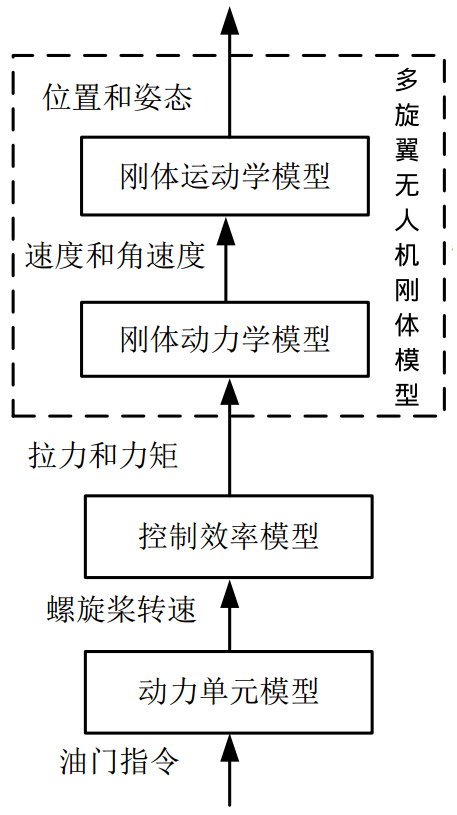
\includegraphics[scale=0.4]{figures/Fig2.1.png}
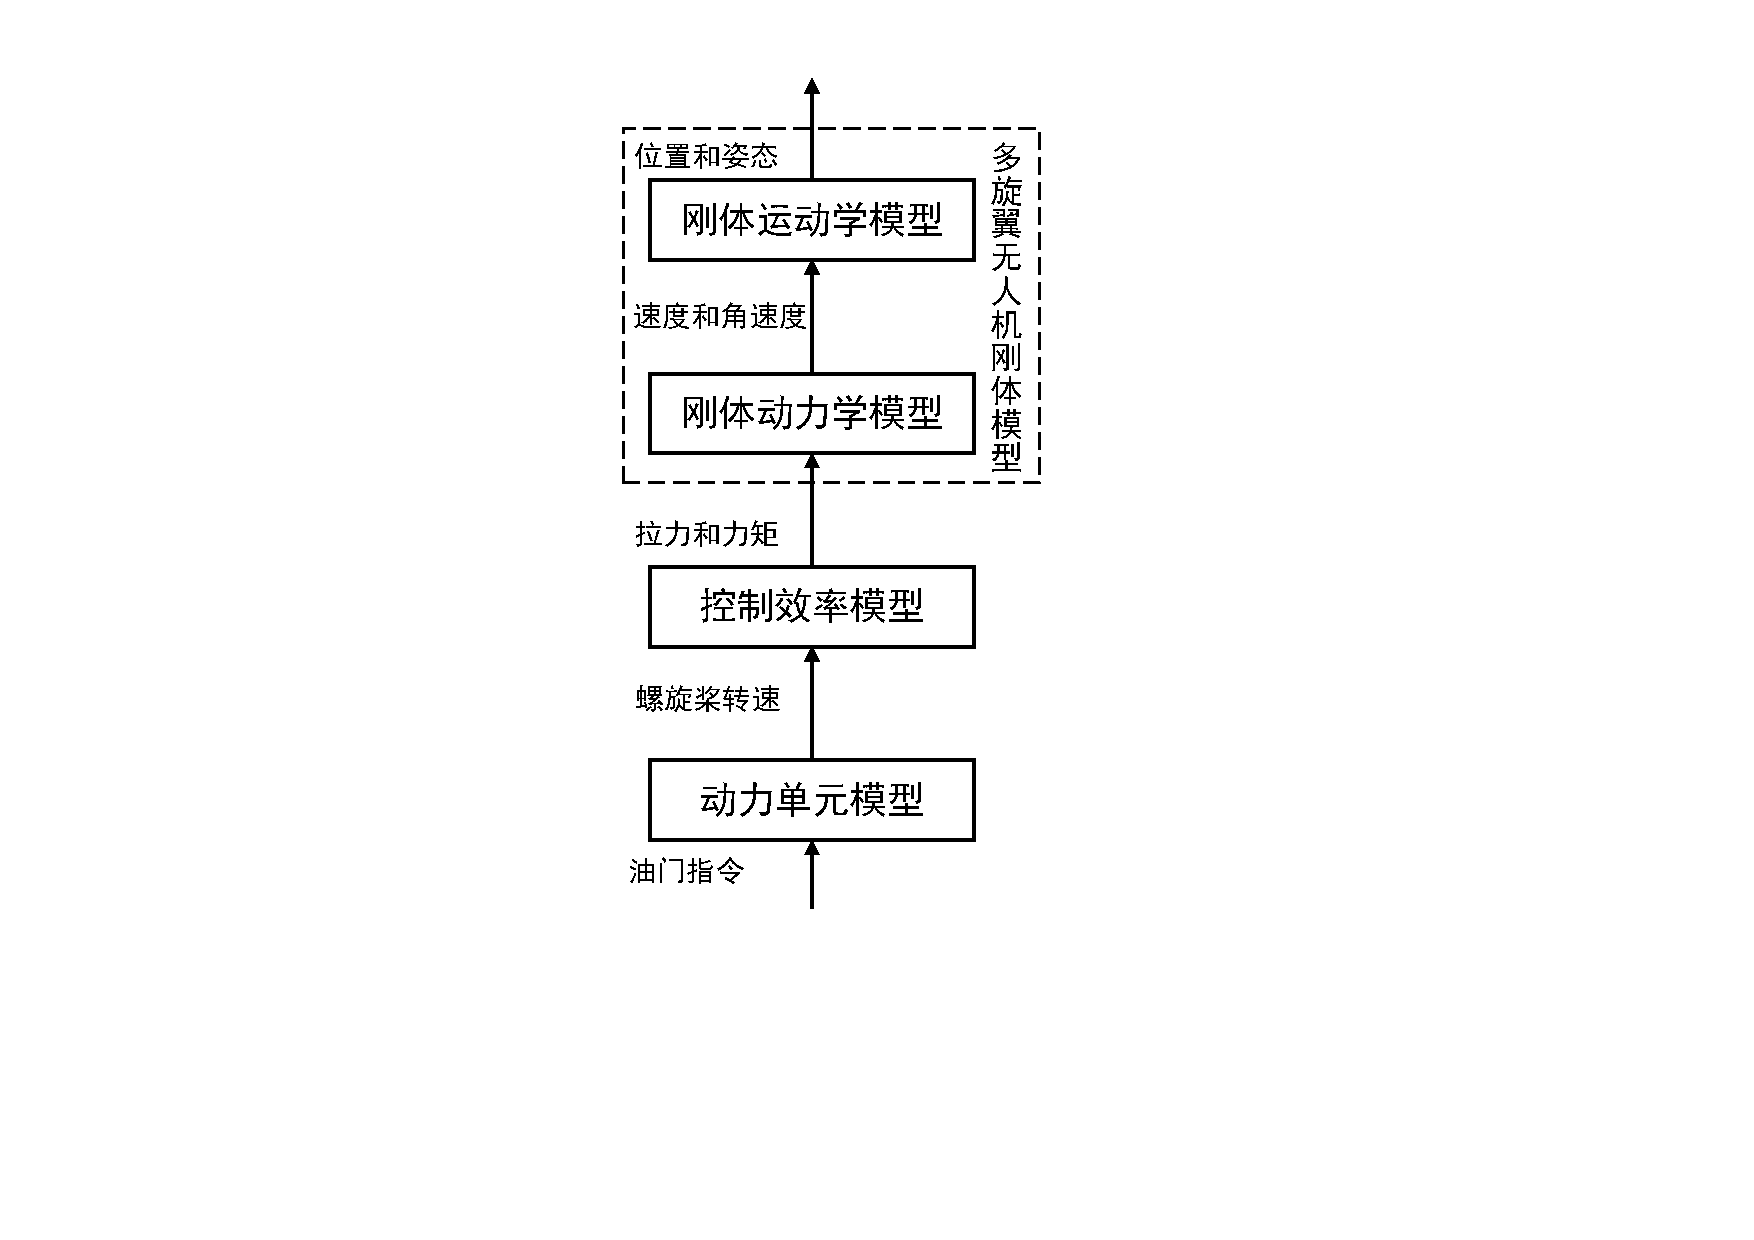
\includegraphics[scale=0.8,,angle=-90]{figures/Fig2-1.pdf}
\caption{多旋翼无人机模型}
\label{fig2.1}
\end{figure}

\subsection{坐标系定义与坐标变换}
多旋翼无人机的空间运动主要分为:质心运动和绕质心的运动,因而在描述任意时刻的空间运动时需要6个自由度:3个质心运动和3个角运动。在进行多旋翼无人机建模之前首先应该选择合适的坐标系,可以方便、准确的表示多旋翼无人机的空间状态和受力情况。本文在进行多旋翼无人机建模时主要用到连个坐标系:固联于无人机的机体坐标系和固定于无人机起飞点的地面坐标系,如图\ref{fig2.2}所示。\\
(1)机体坐标系$\boldsymbol{O} \boldsymbol{x}_b \boldsymbol{y}_b \boldsymbol{z}_b$

机体坐标系原点定义在多旋翼无人机质心上,$\boldsymbol{O} \boldsymbol{x}_b$平行于无人机前后旋翼,指向无人机前进的方向;$\boldsymbol{O} \boldsymbol{z}_b$位于无人机纵向平面,垂直向下;$\boldsymbol{O} \boldsymbol{y}_b$垂直于无人机纵向平面,方向根据右手定则确定。 \\ 
(2)地面坐标系$\boldsymbol{O} \boldsymbol{x}_e \boldsymbol{y}_e \boldsymbol{z}_e$

地面坐标系远点固定于无人机起飞位置,$\boldsymbol{O} \boldsymbol{x}_e$位于地平面内并指向无人机前进方向;$\boldsymbol{O} \boldsymbol{z}_e$垂直与地面并指向地心;$\boldsymbol{O} \boldsymbol{y}_e$位于地面平内,方向根据右手定则确定。

\begin{figure}[h]
\centering
%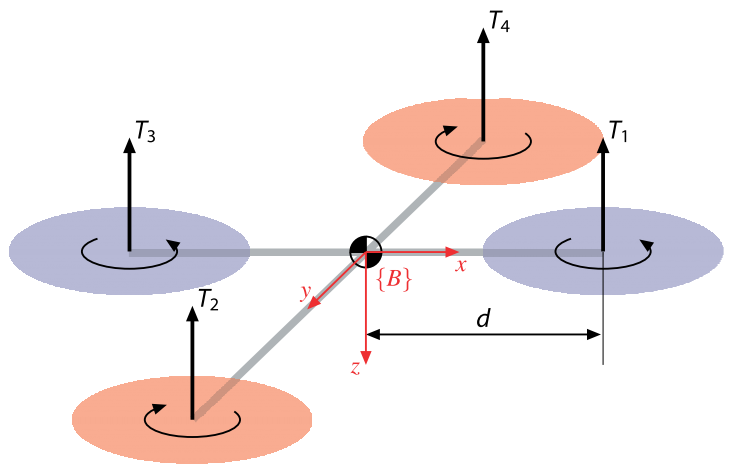
\includegraphics[scale=0.5]{figures/Fig2.2.png}
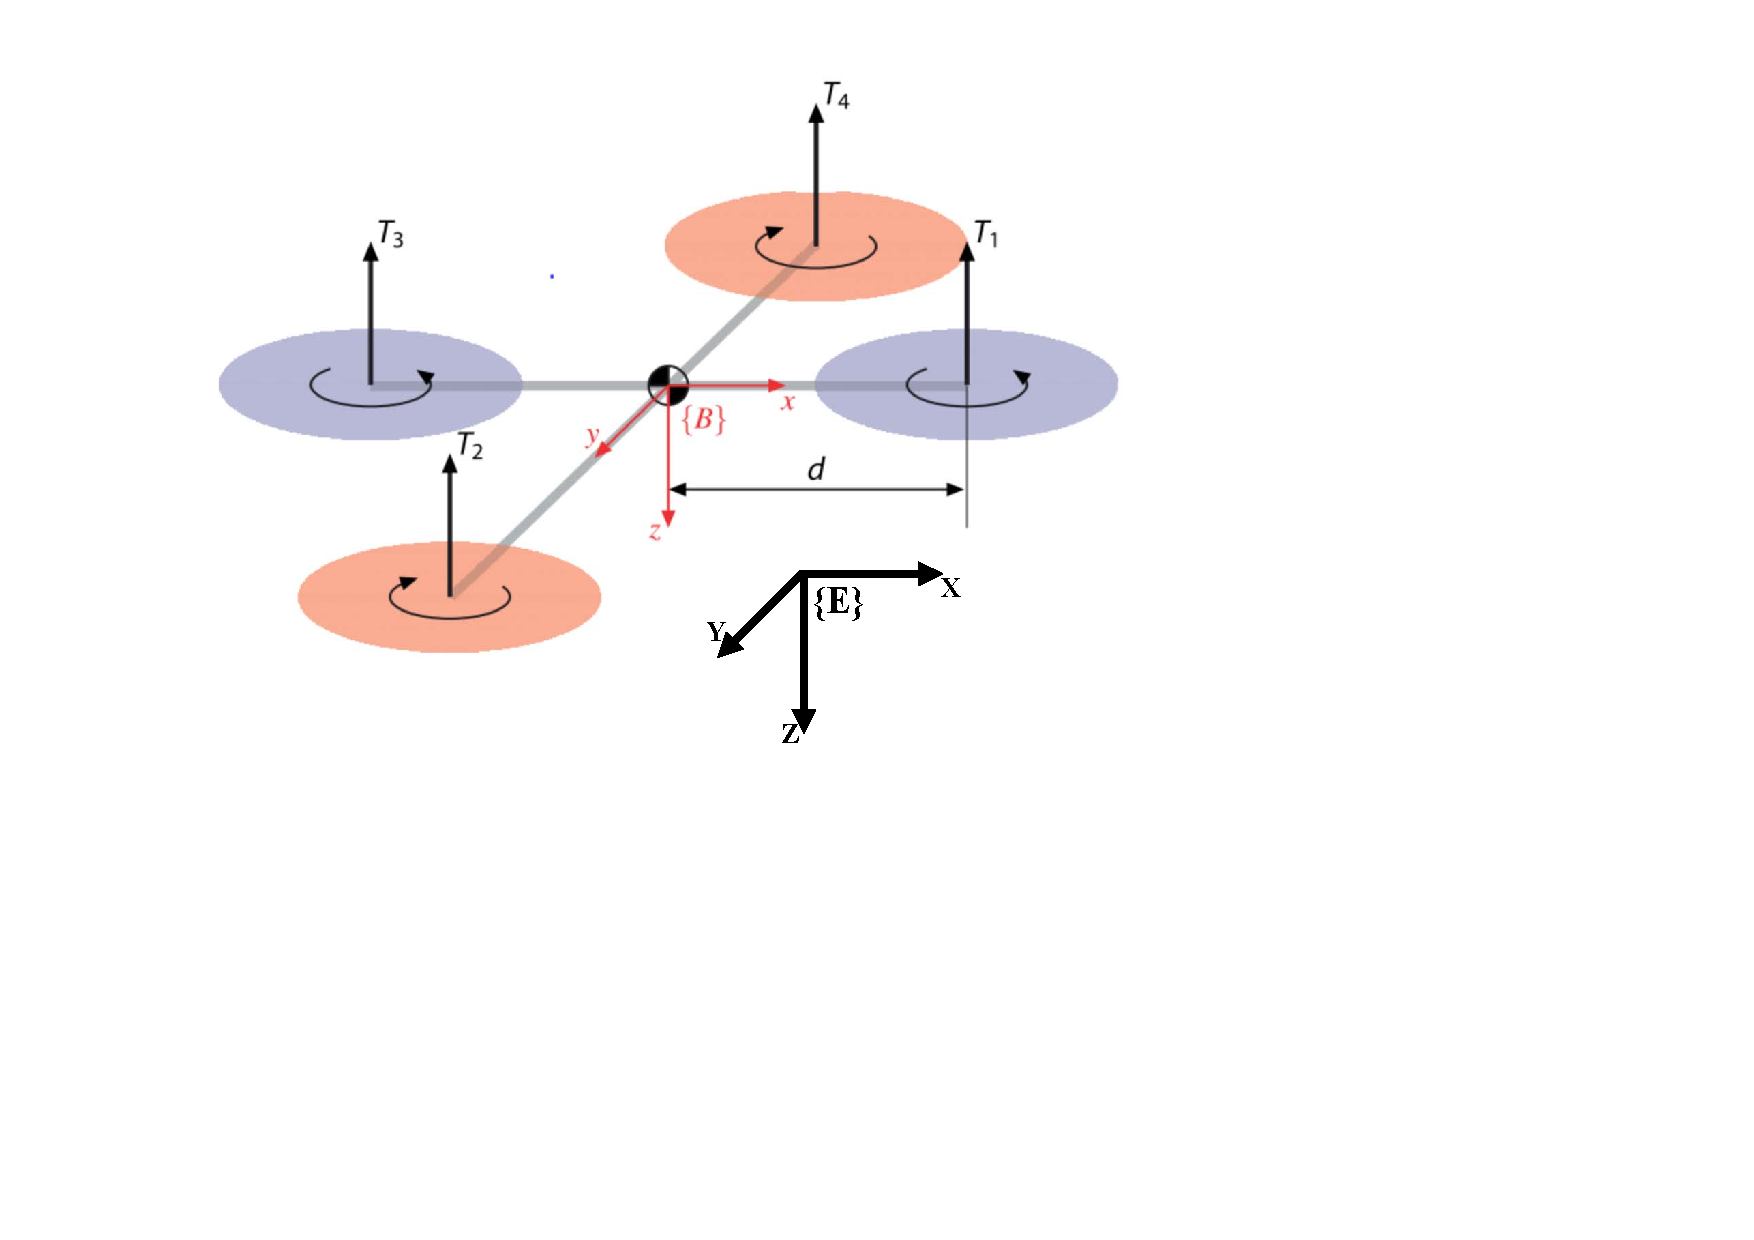
\includegraphics[scale=0.7,angle=-90]{figures/Fig2-2.pdf}
\caption{多旋翼无人机坐标系定义}
\label{fig2.2}
\end{figure}

为了便于描述无人机的空间运动状态,必须选择合适的坐标系,例如选择使用机体坐标系描述空间绕质心的运动,使用地面坐标系描述空间质心运动。当不同坐标系之间需要进行坐标转换,如将机体坐标系受到的螺旋桨拉力转换到地面坐标系分析质心运动。因而,坐标转换是无人机建模不可获取的一部分。一般机体坐标系与地面坐标系之间的转换关系可以由三个姿态角表示,偏航角$\psi$,俯仰角$\theta$和滚转角$\phi$。\\
1).俯仰角$\theta$:机体坐标系$\boldsymbol{O} \boldsymbol{x}_b$轴与地平面之间的夹角,沿$\boldsymbol{O} \boldsymbol{y}_b$轴顺时针旋转抬头为正。\\
2).滚转角$\phi$:机体坐标系$\boldsymbol{O} \boldsymbol{z}_b$与通过机体坐标系$\boldsymbol{O} \boldsymbol{x}_b$轴的铅垂面之间的夹角,沿$\boldsymbol{O} \boldsymbol{x}_b$轴顺时针旋转向右滚转为正。\\
3).偏航角$\psi$:机体坐标系$\boldsymbol{O} \boldsymbol{x}_b$轴在地平面的投影与地面坐标系$\boldsymbol{O} \boldsymbol{x}_e$的夹角,沿$\boldsymbol{O} \boldsymbol{z}_b$轴顺时针旋转右偏为正。

地面坐标系到机体坐标系的转换可以通过欧拉转动定理绕三轴连续转动得到,首先绕地面坐标系$\boldsymbol{O} \boldsymbol{z}_e$转动偏航角$\psi$,得到过度坐标系$\boldsymbol{O} \boldsymbol{x}^{'} \boldsymbol{y}^{'} \boldsymbol{z}^{'}$;之后再由过度坐标系绕$\boldsymbol{O} \boldsymbol{y}^{'}$旋转俯仰角$\theta$,得到过度坐标系$\boldsymbol{O} \boldsymbol{x}^{''} \boldsymbol{y}^{''} \boldsymbol{z}^{''}$;最后由过度坐标系$\boldsymbol{O} \boldsymbol{x}^{''} \boldsymbol{y}^{''} \boldsymbol{z}^{''}$绕$\boldsymbol{O} \boldsymbol{x}^{''}$旋转滚转角$\phi$。则从地面坐标系到机体坐标系的旋转矩阵$\boldsymbol{R}_{BE}$为
\begin{equation}
\label{equ2.1}
\begin{aligned}
\boldsymbol{R}_{BE} 
&= \boldsymbol{R}(\boldsymbol{\phi}) \boldsymbol{R}(\boldsymbol{\theta}) \boldsymbol{R}(\boldsymbol{\psi}) \\ 
&= 
\begin{bmatrix}
\cos\theta \cos\psi & \cos\theta \sin\psi & -\sin\theta \cr
\sin\theta \cos\psi \sin\phi - \sin\psi \cos\phi & \sin\theta \sin\psi \sin\phi + \cos\psi \cos\phi & \cos\theta \sin\phi \cr
\sin\theta \cos\psi \cos\phi + \sin\psi \sin\phi & \sin\theta \sin\psi \cos\phi - \cos\psi \sin\phi & \cos\theta \cos\phi \cr
\end{bmatrix}
\end{aligned}
\end{equation}

\subsection{多旋翼无人机刚体模型}
在进行多旋翼无人机刚体建模前,首先对无人机做出如下假设
\begin{enumerate}  [itemindent=1em,label={(\arabic*)}]
\item 假设多旋翼无人机是刚体。
\item 假设多旋翼无人机的质量和转动惯量保持不变。
\item 假设多旋翼无人机的几何中心和重心重合。
\item 假设多旋翼无人机只受重力和螺旋桨的拉力。
\item 假设奇数编号的螺旋桨逆时针转动,偶数编号螺旋桨顺时针转动
\end{enumerate}
首先进行刚体运动学建模,刚体运动学模型描述了多旋翼无人机运动状态的变化。\\
(1) 质心运动学模型

研究地面坐标系下无人机的位置$\boldsymbol{P}_e = [X,Y,Z]^T$的变化,分解到三轴坐标上有。
\begin{equation}
\label{equ2.2}
\begin{aligned}
\dot{\boldsymbol{P}}_e &= \boldsymbol{V}_e \\
\begin{bmatrix}
\dot{X} \cr \dot{Y} \cr \dot{Z} \cr
\end{bmatrix}
&=
\begin{bmatrix}
V_x \cr V_y \cr V_z \cr
\end{bmatrix}
\end{aligned}
\end{equation}
(2) 质心转动模型

研究姿态角速率$\dot{\boldsymbol{\Theta}}=[\dot{\theta},\dot{\psi},\dot{\phi}]^T$与机体坐标系下的转动角速率$\boldsymbol{\omega}_b=[\omega_x , \omega_y , \omega_z]^T$的关系。根据地面坐标系与机体坐标系之间的变换关系有。
\begin{equation}
\label{equ2.3}
\begin{aligned}
\boldsymbol{\omega}_b & = \boldsymbol{R}_{EB} \dot{\boldsymbol{\psi}}+\boldsymbol{R}(\boldsymbol{\phi}) \dot{\boldsymbol{\theta}}+ \dot{\boldsymbol{\phi}} 
\\
\begin{bmatrix}
\omega_x \cr \omega_y \cr \omega_z \cr
\end{bmatrix}
& =
\begin{bmatrix}
0 & -\sin \theta & 1 \cr
\cos \phi & \cos \theta \sin \phi & 0 \cr
-\sin \phi & \cos \theta \cos \phi & 0 \cr
\end{bmatrix}
\begin{bmatrix}
\dot{\theta} \cr \dot{\psi}  \cr  \dot{\phi} \cr
\end{bmatrix}
\end{aligned}
\end{equation}
(3)质心动力学模型

质心动力学模型研究无人机受力与质心运动的关系。设机体坐标系下所有螺旋桨产生的总拉力$\boldsymbol{T}_b=[0,0,T]^{T}$,无人机受到的重力在世界坐标系下表示为$\boldsymbol{G}_e=[0,0,mg]^T$,则无人机的质心运动方程可以表示为
\begin{equation}
\label{equ2.4}
\begin{aligned}
m\boldsymbol{V}_e &= \boldsymbol{G}_e -  \boldsymbol{R}_{EB} \boldsymbol{T}_b
\end{aligned}
\end{equation}
(4)绕质心转动动力学模型

绕质心转动的动力学模型研究无人机所受力矩与其空间转动的关系。设无人机在机体坐标系下的转动惯量为
\begin{equation}
\label{equ2.5}
\boldsymbol{I}_b = 
\begin{bmatrix}
I_x & 0 & 0 \cr
0 & I_y & 0 \cr
0 & 0 & I_z \cr
\end{bmatrix}
\end{equation}
假设无人机受到的总力矩在世界坐标系下为$\boldsymbol{M}_e=[M_x,M_y,M_z]^T$,根据矢量绝对导数与相对导数关系,由角动量定理得
\begin{equation}
\label{equ2.6}
\begin{aligned}
\boldsymbol{M}_e &= {d\boldsymbol{H}_e \over dt} = {d\boldsymbol{H}_b \over dt} +  \boldsymbol{\omega}_b \times \boldsymbol{H}_b 
\\
\boldsymbol{M}_e &= \boldsymbol{I}_b \dot{\boldsymbol{\omega}}_b +\boldsymbol{\omega}_b \times \boldsymbol{I}_b \boldsymbol{\omega}_b 
\end{aligned}
\end{equation}
以上公式\eqref{equ2.2},\eqref{equ2.3},\eqref{equ2.4},\eqref{equ2.6}组成了多旋翼无人机的非线性刚体模型。

\subsection{多旋翼无人机控制效率模型}
多旋翼无人机控制效率模型研究无人机机型布局与螺旋桨的拉力和力矩分配的关系。以十字型四旋翼无人机为例,已知第$i$个螺旋桨的拉力为$\boldsymbol{F}_i$与电机转速$\omega_i$关系为$\boldsymbol{F}_i = c_T \omega_i^2$,总拉力为
\begin{equation}
\label{equ2.7}
\boldsymbol{T}_b = \sum\limits_{i=1}^4 \boldsymbol{F}_i =  \sum\limits_{i=1}^4 c_T \omega_i^2
\end{equation}
四旋翼无人机机臂长$d$,螺旋桨对机体坐标系三轴产生的力矩为,
\begin{equation}
\label{equ2.8}
\begin{aligned}
M_x &= d c_T \left( \omega_4^2 - \omega_2^2\right)
\\
M_y &= d c_T \left( \omega_1^2 - \omega_3^2\right)
\\
M_z &= d c_M \left( \omega_1^2 - \omega_2^2 + \omega_3^2 - \omega_4^2\right)
\end{aligned}
\end{equation}
公式\eqref{equ2.7},\eqref{equ2.8}中$c_T $表示与螺旋桨类型相关的常量,$c_M$表示螺旋桨反扭力常数,将以上两公式进行整理可以得到无人机动力分配模型
\begin{equation}
\label{equ2.9}
\begin{bmatrix}
T \cr M_x \cr M_y \cr M_z \cr 
\end{bmatrix}
=
\begin{bmatrix}
c_T & c_T & c_T & c_T  \cr
0 & -d c_T & 0 & d c_T \cr
d c_T & 0 & -d c_T & 0 \cr
c_M & c_M & c_M & c_M  \cr
\end{bmatrix}
\begin{bmatrix}
\omega_1^2 \cr \omega_2^2 \cr \omega_3^2 \cr \omega_4^2 \cr
\end{bmatrix}
\end{equation}


\subsection{多旋翼无人机动力单元模型}
多旋翼无人机一般选用直流无刷电机,无刷电机微分方程为
\begin{equation}
\label{equ2.10}
\begin{aligned}
u &= iR + L {di \over dt} + k_e \omega
\\
J_m {d\omega \over dt} &= M_m - M_{load}
\end{aligned}
\end{equation}
其中$u$表示电机电压,$i$为电机电流,$\omega$表示电机旋转角速度,$R$表示电机等效电阻,$L$表示电机线圈电感,$k_e$表示电机反电动势系数,$J_m$表示电机线圈的轴向转动惯量,$M_m=k_m i$表示电机输出力矩,$M_{load}$表示电机负载力矩。由于电机线圈电感较小,省略后可以化简得到多旋翼无人机动力单元模型
\begin{equation}
\label{equ2.11}
\begin{aligned}
i &= {(u-k_e \omega) \over R }
\\
J_m {d \omega \over dt} &= k_m{u \over R } - {k_e k_m \omega \over R} - M_{load}
\end{aligned}
\end{equation}

%2.2
\section{多旋翼无人机控制算法研究}
为了更好的控制飞行器运动,采用串级PID进行控制策略,分为两个控制器位置控制器和姿态控制器。位置控制器为外环,负责控制多旋翼无人机的位置;姿态控制器为内环,负责控制多旋翼无人机的姿态角。由内外环控制实现多旋翼飞行器的升降、悬停和侧飞等飞行模态,控制系统结构狂徒如图\ref{fig2.3}所示。
\begin{figure}[h]
\centering
%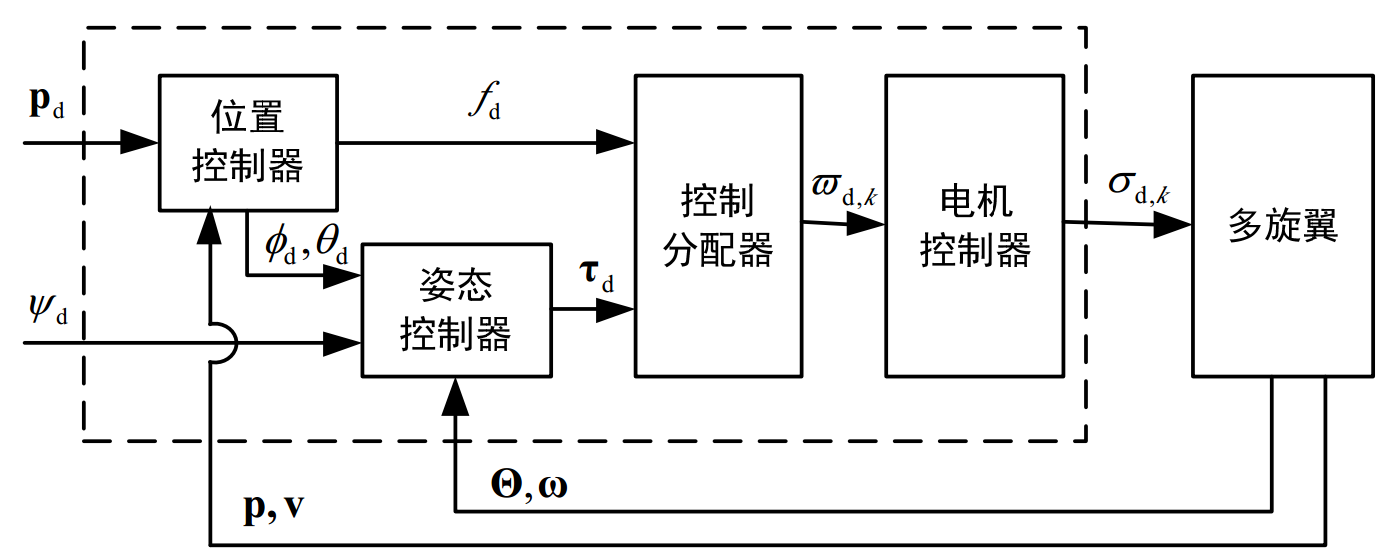
\includegraphics[scale=0.3]{figures/Fig2.3.png}
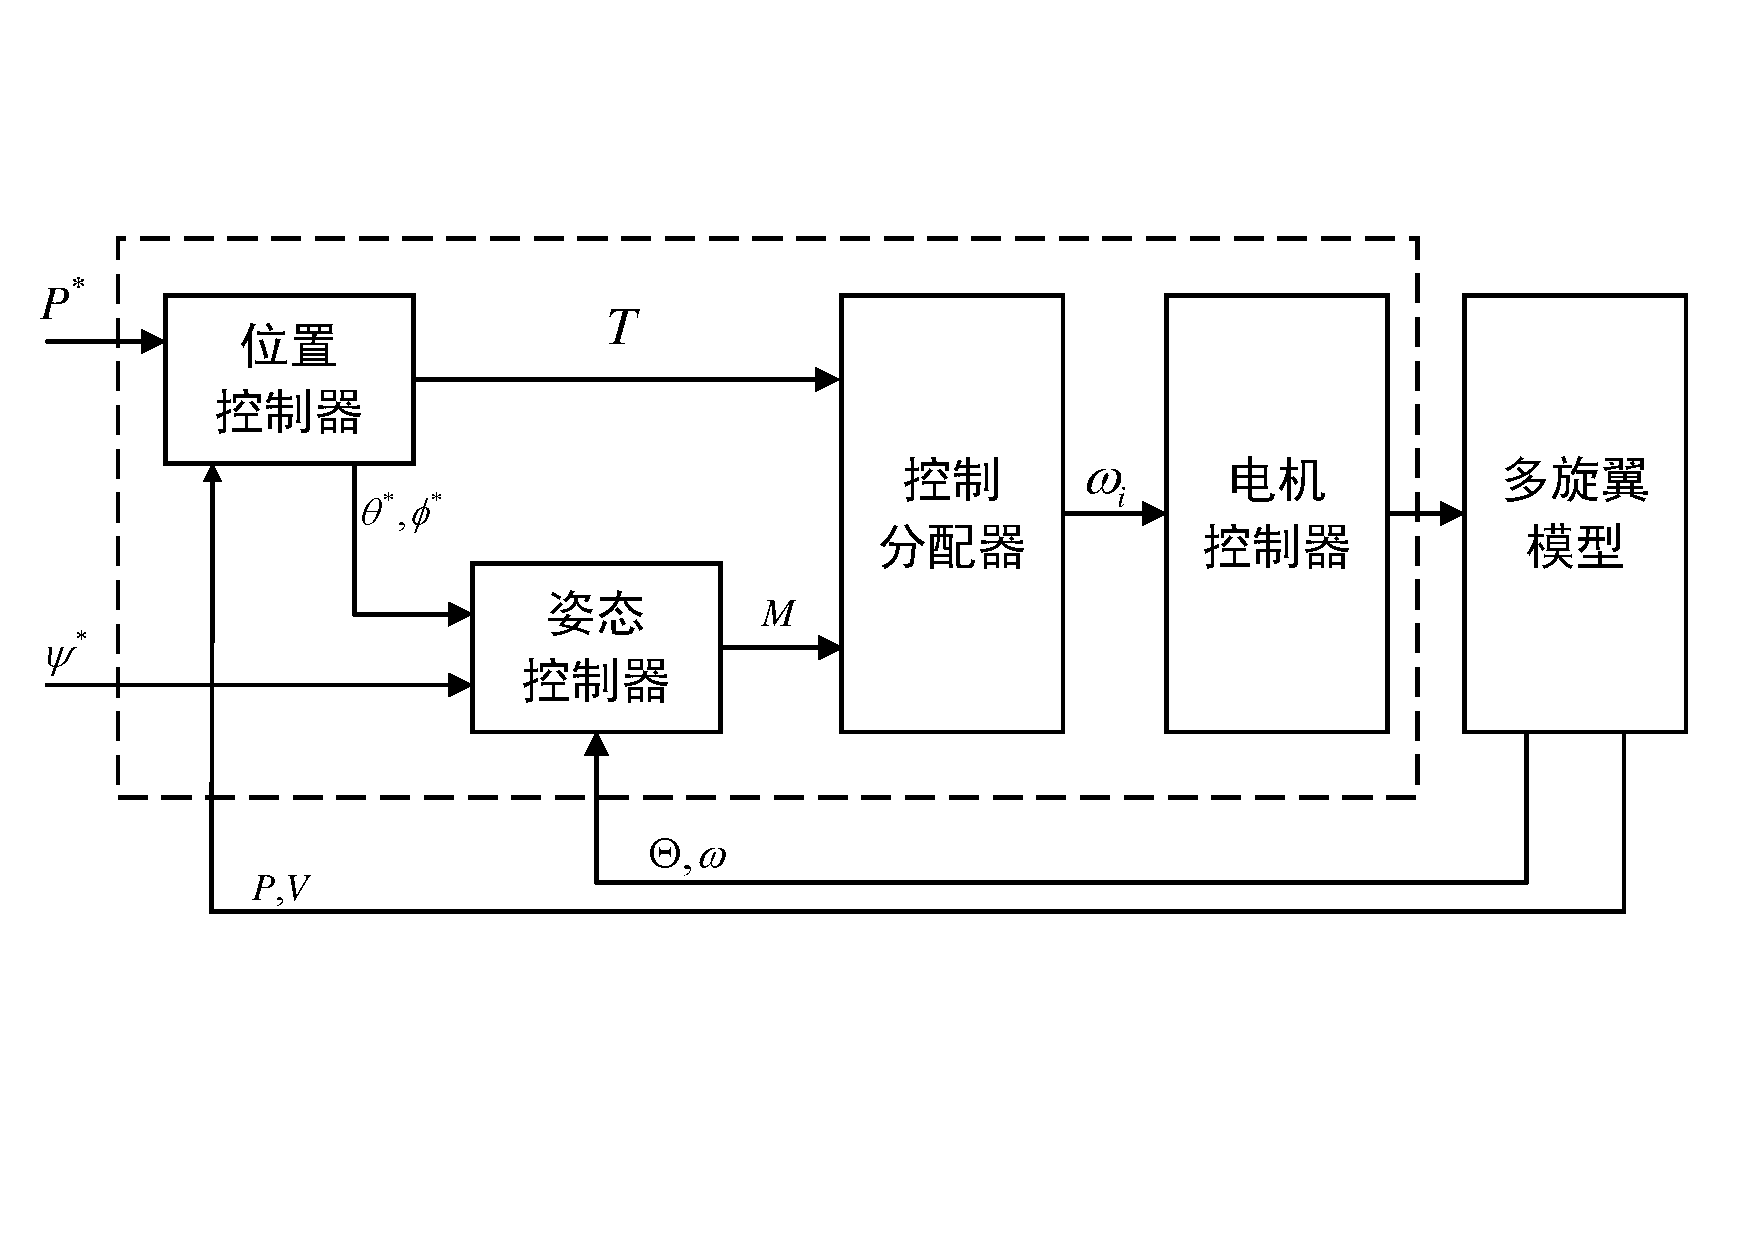
\includegraphics[scale=0.5,angle=-90]{figures/Fig2-3.pdf}
\caption{多旋翼无人机闭环控制框图}
\label{fig2.3}
\end{figure}

\subsection{姿态控制器}
多旋翼无人机的姿态角直接影响无人机的飞行状态,对于内环姿态控制器,根据方程\eqref{equ2.5}可知多旋翼飞行器绕质心转动的动力学模型为二阶系统,因而在姿态控制回路引入比例-微分控制器进行调节,并将控制通道解耦为俯仰/滚转通道和偏航通道。对于俯仰/滚转通道,多旋翼无人机的俯仰、滚转运动对称,因而以俯仰通道为例介绍,设计比例-微分控制器
\begin{equation}
\label{equ2.12}
\begin{aligned}
M_x &= K_{p\theta} \left( \theta^* - \theta \right) + K_{d\theta} \left( \dot{\theta}^* -  \dot{\theta} \right)
\end{aligned}
\end{equation}
其中$\theta^*$、$\dot{\theta}$表示反馈的姿态角和姿态角速率,$\theta^*$表示期望俯仰角,由位置控制器给出。$ \dot{\theta}^*$通常较小可以忽略。

对于偏航通道,同样采用比例-微分控制器
\begin{equation}
\label{equ2.13}
M_z = K_{p\psi} \left( \psi^* - \psi \right) + K_{d\psi} \left( \dot{\psi}^* -  \dot{\psi} \right)
\end{equation}
其中$\psi$、$\dot{\psi}$表示反馈的姿态角和姿态角速率。不同于俯仰/滚转通道,$\psi^*$表示的期望俯仰角不由位置控制器给出,而是根据规划的轨迹或外部遥控装置直接给出。$ \dot{\psi}^*$通常较小可以忽略。

\subsection{位置控制器}
对多旋翼无人机刚体运动学模型\eqref{equ2.3},\eqref{equ2.4}进行线性化近似可知,多旋翼无人机的水平运动影响俯仰/滚转姿态角变化,高度运动影响无人机推力变化。对于水平运动,$x$,$y$方向的运动是等价的,以x方向运动为例,设计比例控制器约束无人机的期望速度
\begin{equation}
\label{equ2.14}
v_x^* =  K_{px} \left( p_x^* - p_x \right)
\end{equation}
其中$p_x $表示反馈的$x$方向位置,$p_x^*$表示$x$方向的期望位置,$v_x^*$表示$x$方向的期望速度。根据\eqref{equ2.3}的现行近似模型可知,为了使机体产生沿$x$方向的运动,需要产生俯仰角,有
\begin{equation}
\label{equ2.15}
f_x = T \sin\theta \simeq T \theta
\end{equation}
根据方程\eqref{equ2.15}设计比例控制器
\begin{equation}
f_x = K_{vx} \left(  v_x^* - v_x \right)
\end{equation}
联立方程\eqref{equ2.14},\eqref{equ2.15}可以得到期望的俯仰姿态角$\theta^*$
\begin{equation}
\label{equ2.16}
\theta^* = K_{vx} \left( K_{px} \left( p_x^* - p_x \right) - v_x \right)
\end{equation}

对于高度控制器,设计比例-微分控制器调节多旋翼无人机的推力
\begin{equation}
\label{equ2.17}
T = K_{pz} \left( z^* -z  \right) + K_{dz} \left( \dot{z}^* - \dot{z}  \right) + G_0
\end{equation}
其中,$z^*$表示目标高度,$z$,$\dot{z}$表示无人机反馈的高度位置和速度。$G_0$是前馈控制量,抵消重力的影响,避免高度控制中的定常干扰。

%2.3
\section{ 数学仿真验证}



\section{本章小结}



\iffalse
%2.4
%\section{Weighted Gauss-Newton Optimization on Lie-Manifolds}
Two images are aligned by Gauss-Newton minimization of the photometric error
\begin{equation}
E(\xi)=\sum( I_{ref}(p_{i} - I( \omega( p_{i},D_{ref}(p_{i}),\xi ) ))^{2}
\end{equation}
which gives the maximum-likelihood estimator for ${\mathbf{\xi }}$ assuming Gaussian residuals. We use a left-compositional formulation. Starting with an initial estimate ${{\mathbf{\xi }}^{{\mathbf{(0)}}}}$, in each iteration a left-multiplied increment $\delta {{\mathbf{\xi }}^{{\mathbf{(n)}}}}$ is computed by solving for the minimum of Gauss-Newton second-order approximation of E.
\begin{equation}
\delta\xi^{n}=-(J^{T}J)^{-1}J^{T}r(\xi^{n}) \ with \  \left. J=\frac{\partial r(\varepsilon\circ\xi^{n})}{\partial \varepsilon} \right|_{\varepsilon=0}
\end{equation}

where ${\mathbf{J}}$ is the derivative of the stacked residual vector ${ r=(r_{1},...,r_{n})^{T} }$ with respect to a left-multiplied increment, and ${{\mathbf{J}}^{\mathbf{T}}}{\mathbf{J}}$ the Gauss-Newton approximation of the Hessian of $E$. The new estimate is then obtained by multiplication with the computed update

\begin{equation}
\xi ^{(n + 1)} = \delta \xi ^{(n)} \circ \xi ^{(n)}
\end{equation}

In order to be robust to outliers arising from occlusions or reflections, different weighting-schemes have been proposed by [7].

\begin{equation}
E(\xi)=\sum\limits_i \omega_{i}(\xi)r_{i}(\xi)
\end{equation}
and the update is computed as

\begin{equation}
\delta {\xi ^{(n)}} =  - (J^{T}WJ)^{ - 1}J^{T}W_{r}({\xi ^{(n)}})
\end{equation}

Assuming the residuals to be independent, the last iteration ${({J^T}WJ)^{ - 1}}$ is an estimate for the covariance   of a left-multiplied error onto the final result. The default type-implementation in g2o assumes right-multiplication [8].

\begin{equation}
\xi ^{(n)} = \varepsilon  \circ \xi _{true} \ with \ \varepsilon \sim N(0,\sum \varepsilon  )
\end{equation}
\fi



